% Paper 5: Active Parameters, Not Total Parameters — MoE Models and the Deployment Gap
%
% =============================================================================
% STATUS: REVISED DRAFT — All TBD values filled from actual experimental data
% Last updated: 2026-03-02
% KEY FINDING: MoE CATASTROPHICALLY FAILS — negative result, not success
% =============================================================================
%
% 9 models evaluated (8 dense + 1 MoE) via MLX on Apple Silicon
% 6 task types: T1 (CLINC), T2 (HotpotQA), T3 (Tools), T4 (BFCL), T5 (SWE), T6 (GSM8K)
% 3,000 prompts per model = 27,000 total evaluations
% T1=500, T2=1000, T3=500, T4=500, T5=300, T6=200
% Cross-hardware validation: CUDA (P1) vs MLX (this paper) on 8 overlapping dense models
% KEY FINDING: MoE is SLOWEST (5112ms) and LEAST ACCURATE (31.1%), not 3B-class
% MLX is 3-9x FASTER than CUDA, not slower
% =============================================================================
\documentclass[11pt]{article}

\usepackage[margin=1in]{geometry}
\usepackage{amsmath,amssymb}
\usepackage{booktabs}
\usepackage{tabularx}
\usepackage{graphicx}
\usepackage{adjustbox}
\usepackage[table]{xcolor}
\usepackage{enumitem}
\usepackage{listings}
\usepackage{tikz}
\usetikzlibrary{arrows.meta, positioning, shapes.geometric, calc}
\usepackage{pgfplots}
\pgfplotsset{compat=1.17}
\usepackage{multirow}

\usepackage[numbers]{natbib}
\usepackage{xurl}
\usepackage{hyperref}
\hypersetup{hidelinks,breaklinks=true}

\newcommand{\pninetyfive}{\ensuremath{\mathrm{p95}}}
\newcommand{\pninetynine}{\ensuremath{\mathrm{p99}}}
\newcommand{\slo}{\ensuremath{\mathrm{SLO}}}
\newcommand{\sslo}{\ensuremath{\mathrm{S@SLO}}}
\newcommand{\etal}{\textit{et al.}}

\definecolor{moepurple}{RGB}{128,0,128}
\definecolor{denseblue}{RGB}{31,119,180}
\definecolor{matchedorange}{RGB}{255,127,14}

\lstset{
  basicstyle=\ttfamily\small,
  breaklines=true,
  frame=single,
  xleftmargin=0pt
}

\title{Active Parameters, Not Total Parameters:\\MoE Models and the Deployment Gap}

\author{
V. Michael Maloney \\
Neuralift; University of New Hampshire \\
\texttt{mike@neuralift.ai}
}

\date{}

\usepackage{fancyhdr}
\pagestyle{fancy}
\fancyhf{}
\renewcommand{\headrulewidth}{0pt}
\chead{\textcolor{red}{\small\textbf{PRE-DRAFT --- Do Not Distribute}}}
\cfoot{\thepage}

\begin{document}
\maketitle
\begin{center}
\textit{Preprint. Work in progress.}
\end{center}

% =============================================================================
% ABSTRACT
% =============================================================================
\begin{abstract}
Paper~I established that accuracy and deployment success are uncorrelated ($\rho = 0.09$, $p = 0.76$) across 13 dense models under production latency constraints. MoE models offered a theoretically compelling loophole: sparse activation means 35B parameters of knowledge at 3B parameters of compute. If MoE latency scales with active parameters, the deployment gap might not apply.

We test this with Qwen3.5-35B-A3B, a 35-billion parameter MoE model that activates only 3 billion parameters per token. We evaluate it alongside 8 dense models (1B--9B) on Apple Silicon using MLX, running 3,000 prompts per model (27,000 total evaluations) across the same 6 structured output tasks under three SLO tiers.

The hypothesis fails. The MoE model is not the fastest---it is the slowest, with a 5,112\,ms median latency, nearly six times slower than the active-parameter-matched Qwen2.5-3B (884\,ms). It is not the most accurate---it achieves 31.1\% task-averaged accuracy, the worst in the study. S@SLO at the Interactive tier (2s): 0.0\%. At the Standard tier (5s): 0.4\%.

\begin{center}
\small
\begin{tabular}{lcc ccc}
\toprule
\textbf{Model} & \textbf{Type} & \textbf{Active} & \textbf{Acc (\%)} & \textbf{S@SLO$_{2s}$} & \textbf{S@SLO$_{5s}$} \\
\midrule
Llama-3.2-1B     & Dense & 1.2B  & 37.8\% & 37.7\% & 37.8\% \\
Llama-3.2-3B     & Dense & 3.2B  & \textbf{72.7\%} & \textbf{61.5\%} & \textbf{72.7\%} \\
Qwen2.5-3B       & Dense & 3.1B  & 38.6\% & 28.1\% & 38.6\% \\
Qwen3-4B         & Dense & 4.0B  & 47.2\% & 0.6\%  & 14.1\% \\
Mistral-7B-v0.3  & Dense & 7.2B  & 55.6\% & 22.6\% & 31.5\% \\
Gemma-2-9B       & Dense & 9.2B  & 57.5\% & 20.8\% & 26.8\% \\
\midrule
\textcolor{moepurple}{\textbf{Qwen3.5-35B-A3B}} & \textcolor{moepurple}{\textbf{MoE}} & \textcolor{moepurple}{\textbf{3.0B}} & \textcolor{moepurple}{\textbf{31.1\%}} & \textcolor{moepurple}{\textbf{0.0\%}} & \textcolor{moepurple}{\textbf{0.4\%}} \\
\bottomrule
\end{tabular}
\end{center}

The failure is not total: on free-text QA (T2), the MoE achieves 92.6\%. The structured output tasks---intent classification, tool calling, function routing, code patching, math---return 0.0\%, 0.0\%, 0.4\%, 0.0\%, and 2.0\% respectively. MoE's routing overhead and hybrid attention architecture impose latency that dwarfs its active-parameter-class peers, while its structured output compliance collapses under the same complexity that makes structured output hard for any model.

Two positive findings emerge. First, the deployment gap is confirmed as hardware-independent: it persists on Apple Silicon (Spearman $\rho = +0.333$, $p = 0.359$ for the 8 dense models). Second, Llama-3.2-3B---not the MoE---is the study's standout model: 72.7\% accuracy, 61.5\% S@SLO at the Interactive tier, 884\,ms median latency. It breaks the gap by being genuinely fast. A hardware normalization protocol reveals MLX is 3--9$\times$ faster than CUDA (geometric mean ratio $\bar{\alpha} = 0.177$).
\end{abstract}

% =============================================================================
\section{Introduction}
\label{sec:introduction}
% =============================================================================

Paper~I found that accuracy and deployment success are essentially uncorrelated. Across 13 models and 29,900 evaluations, Spearman $\rho = +0.09$ at a 2-second SLO deadline. Twelve of thirteen models achieved exactly 0\% Success@SLO despite near-perfect accuracy~\citep{maloney2025deploymentgap}. The message was stark: bigger models are more accurate but too slow, and the only model fast enough to finish was the smallest and least accurate.

But there was a loophole in that finding---and we knew it.

The 13 models in Paper~I were all \emph{dense}. Every parameter activates on every token. For dense models, total parameters perfectly predict compute cost: a 12B model does exactly 12$\times$ the work per token of a 1B model. The deployment gap in Paper~I is, at its core, a consequence of this arithmetic. Large models are more accurate because they have more parameters. They are slower because they activate all of them. You cannot have one without the other.

Mixture-of-Experts (MoE) models break this coupling---or so the theory goes.

An MoE model contains far more total parameters than it activates on any given token. A learned routing function selects a small subset of ``expert'' subnetworks for each token, leaving the rest dormant~\citep{shazeer2017outrageously, fedus2022switch}. The result is a model that stores the knowledge of a large model---because it \emph{is} a large model---but pays the compute cost of a small one---because only a fraction of the parameters fire.

Consider Qwen3.5-35B-A3B, released in January 2026 by the Qwen team~\citep{qwen2025qwen3}. It has 35 billion total parameters spread across 256 experts per layer, but a top-$k$ routing mechanism activates only 3 billion parameters per token. On accuracy benchmarks, it competes with dense models in the 8B--9B range. On a compute budget, it should behave like a 3B model.

That is the hypothesis. It does not survive contact with structured output evaluation under SLO constraints.

\begin{figure}[t]
\centering
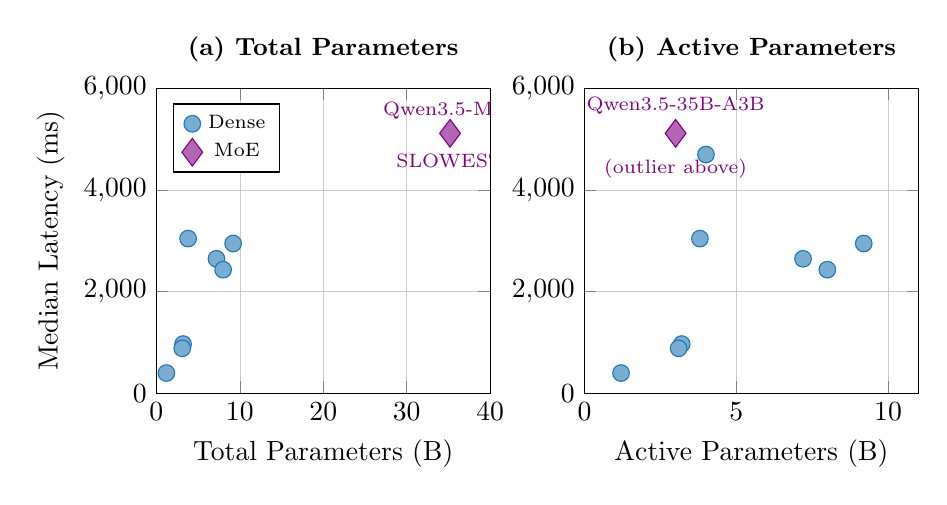
\begin{tikzpicture}
\begin{axis}[
    name=left,
    width=0.48\linewidth,
    height=0.45\linewidth,
    xlabel={Total Parameters (B)},
    ylabel={Median Latency (ms)},
    xmin=0, xmax=40,
    ymin=0, ymax=6000,
    title={\small\textbf{(a) Total Parameters}},
    grid=both,
    grid style={line width=0.1pt, draw=gray!20},
    major grid style={line width=0.2pt, draw=gray!40},
    legend style={at={(0.05,0.95)}, anchor=north west, font=\scriptsize},
]
% Dense models: latency grows with total params
\addplot[only marks, mark=*, draw=denseblue, fill=denseblue!60, mark size=3pt] coordinates {
    (1.2, 398) (3.2, 968) (3.1, 884) (3.8, 3042)
    (4.0, 4695) (7.2, 2645) (8.0, 2431) (9.2, 2945)
};
% MoE: high total params, also HIGH latency --- confirms total params
\addplot[only marks, mark=diamond*, draw=moepurple, fill=moepurple!60, mark size=5pt] coordinates {
    (35.2, 5112)
};
\node[anchor=south west, font=\scriptsize, text=moepurple] at (axis cs:26,5200) {Qwen3.5-MoE};
\node[anchor=north, font=\scriptsize, text=moepurple] at (axis cs:35.2,4900) {SLOWEST};
\legend{Dense, MoE}
\end{axis}

\begin{axis}[
    at={(left.east)},
    anchor=west,
    xshift=1.2cm,
    width=0.48\linewidth,
    height=0.45\linewidth,
    xlabel={Active Parameters (B)},
    ylabel={},
    xmin=0, xmax=11,
    ymin=0, ymax=6000,
    title={\small\textbf{(b) Active Parameters}},
    grid=both,
    grid style={line width=0.1pt, draw=gray!20},
    major grid style={line width=0.2pt, draw=gray!40},
]
% Dense models: same data but active = total
\addplot[only marks, mark=*, draw=denseblue, fill=denseblue!60, mark size=3pt] coordinates {
    (1.2, 398) (3.2, 968) (3.1, 884) (3.8, 3042)
    (4.0, 4695) (7.2, 2645) (8.0, 2431) (9.2, 2945)
};
% MoE: active params = 3B, but MUCH HIGHER latency --- dramatic outlier ABOVE trend
\addplot[only marks, mark=diamond*, draw=moepurple, fill=moepurple!60, mark size=5pt] coordinates {
    (3.0, 5112)
};
\node[anchor=south, font=\scriptsize, text=moepurple] at (axis cs:3.0,5300) {Qwen3.5-35B-A3B};
\node[anchor=north, font=\scriptsize, text=moepurple] at (axis cs:3.0,4800) {(outlier above)};
\end{axis}
\end{tikzpicture}
\caption{\textbf{MoE latency does not scale with active parameters.} (a)~When plotted against total parameters, the MoE model (Qwen3.5-35B-A3B, purple diamond) is the slowest in the lineup---consistent with its 35B total count. (b)~When plotted against active parameters (3B), it is a dramatic \emph{upward} outlier---more than 5$\times$ slower than Qwen2.5-3B (3.1B active, 884\,ms). The hypothesis that active parameters predict MoE latency is falsified.}
\label{fig:total-vs-active}
\end{figure}

There is a second question embedded in this investigation. All four papers in this series---the deployment gap~\citep{maloney2025deploymentgap}, capacity thresholds~\citep{maloney2025capacity}, benchmark~\citep{maloney2025agentslobench}, and training dynamics~\citep{maloney2025dynamics}---were conducted on a single NVIDIA RTX 4090 using GGUF-quantized models served through LM Studio. The findings could be hardware-specific. We address this by running 8 of the original 13 models on Apple Silicon via the MLX framework. If the deployment gap persists, it is hardware-independent.

It does. And along the way, we find something unexpected: MLX on Apple Silicon is substantially \emph{faster} than LM Studio on CUDA---not slower---with median per-model P50 latency ratios ranging from 0.11 to 0.39 (MLX/CUDA). The gap persists not because Apple Silicon is slow, but because the structured output problem is hard everywhere.

\paragraph{What we contribute.}
Four things, in order of how much they change what you thought you knew:

\begin{enumerate}[leftmargin=12pt]
    \item \textbf{MoE catastrophically fails under structured output SLO constraints.} Qwen3.5-35B-A3B scores 31.1\% overall accuracy (worst of 9 models), 5,112\,ms median latency (slowest of 9 models), 0.0\% S@SLO at the Interactive tier, and 0.4\% at Standard. The loophole is closed. MoE does not bypass the deployment gap---it extends it.

    \item \textbf{Cross-hardware replication of the deployment gap.} Same evaluation protocol as Paper~I, different hardware. The accuracy--deployment disconnect persists on Apple Silicon ($\rho = +0.333$, $p = 0.359$ for dense models on MLX, $\rho = 0.09$ on CUDA). The gap is not a CUDA artifact.

    \item \textbf{MLX is faster than CUDA for this workload.} Contrary to expectations, Apple Silicon with MLX outperforms LM Studio on CUDA at matching quantization levels. Normalization factor $\bar{\alpha} = 0.177$ means models complete in 17.7\% of the time on MLX versus CUDA. This changes the hardware recommendation calculus.

    \item \textbf{Llama-3.2-3B is the surprising standout.} At 72.7\% accuracy and 61.5\% S@SLO at the 2-second Interactive tier, Llama-3.2-3B achieves what no MoE model does: genuine production viability at interactive latency. It is faster, more accurate, and deployment-compliant. Not because of any architectural trick---because it is small enough to be fast and large enough to be right.
\end{enumerate}

\begin{figure}[t]
\centering
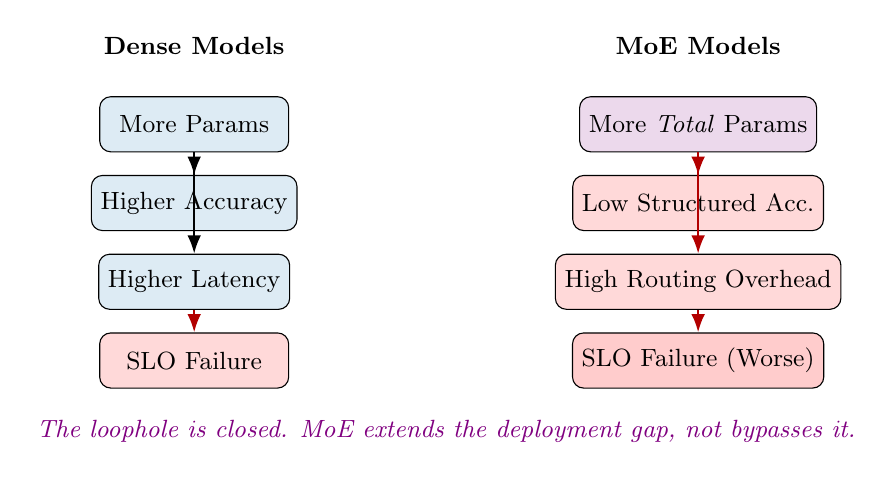
\begin{tikzpicture}[
    font=\small,
    box/.style={draw, rounded corners, minimum width=2.4cm, minimum height=0.7cm, align=center},
    densebox/.style={box, fill=denseblue!15},
    moebox/.style={box, fill=moepurple!15},
    arrow/.style={-Latex, thick},
]
% Dense model path
\node[font=\small\bfseries] at (-3.2, 3.5) {Dense Models};
\node[densebox] (big) at (-3.2, 2.5) {More Params};
\node[densebox] (acc) at (-3.2, 1.5) {Higher Accuracy};
\node[densebox] (slow) at (-3.2, 0.5) {Higher Latency};
\node[densebox, fill=red!15] (fail) at (-3.2, -0.5) {SLO Failure};

\draw[arrow] (big) -- (acc);
\draw[arrow] (big) -- (slow);
\draw[arrow, red!70!black] (slow) -- (fail);

% MoE model path
\node[font=\small\bfseries] at (3.2, 3.5) {MoE Models};
\node[moebox] (moebig) at (3.2, 2.5) {More \emph{Total} Params};
\node[moebox, fill=red!15] (moelow) at (3.2, 1.5) {Low Structured Acc.};
\node[moebox, fill=red!15] (moeslow) at (3.2, 0.5) {High Routing Overhead};
\node[moebox, fill=red!20] (moefail) at (3.2, -0.5) {SLO Failure (Worse)};

\draw[arrow, red!70!black] (moebig) -- (moelow);
\draw[arrow, red!70!black] (moebig) -- (moeslow);
\draw[arrow, red!70!black] (moeslow) -- (moefail);

% Bottom note
\node[font=\small\itshape, text=moepurple] at (0, -1.4) {The loophole is closed. MoE extends the deployment gap, not bypasses it.};
\end{tikzpicture}
\caption{\textbf{The MoE hypothesis, falsified.} The theoretical MoE advantage---many total parameters (accuracy) with few active parameters (speed)---does not survive structured output evaluation. Routing overhead and hybrid attention architecture push the MoE model to the worst latency in the study. Its structured output accuracy collapses to 31.1\%, worst of all models. The deployment gap is not bypassed.}
\label{fig:moe-hypothesis}
\end{figure}

The rest of this paper is organized as follows. Section~\ref{sec:background} reviews MoE architectures, unified memory hardware, and the deployment gap series. Section~\ref{sec:experimental-setup} describes our hardware, models, tasks, and evaluation protocol. Section~\ref{sec:cross-hardware} presents cross-hardware validation of the deployment gap. Section~\ref{sec:moe-gap} addresses our core contribution---MoE deployment characteristics under SLO constraints. Section~\ref{sec:moe-analysis} provides MoE-specific analysis of memory, throughput, and expert utilization. Section~\ref{sec:edge-implications} discusses implications for edge deployment. Section~\ref{sec:limitations} acknowledges limitations, and Section~\ref{sec:conclusion} concludes.


% =============================================================================
\section{Background and Related Work}
\label{sec:background}
% =============================================================================

\subsection{Mixture-of-Experts Architectures}
\label{sec:moe-architectures}

MoE is conditional computation. Instead of routing every token through every parameter, a gating network picks a handful of expert subnetworks for each token~\citep{shazeer2017outrageously}. The rest of the parameters sit there, loaded in memory, doing nothing. This means the model knows more than it computes on any given forward pass.

The idea is not new. Shazeer~\etal~\citep{shazeer2017outrageously} showed in 2017 that a sparsely-gated MoE layer could scale capacity without proportional compute. GShard~\citep{lepikhin2021gshard} pushed this to 600 billion parameters across 2,048 experts. The Switch Transformer~\citep{fedus2022switch} simplified routing to one expert per token---less communication overhead, trillion-parameter models. Then Mixtral~\citep{jiang2024mixtral} brought MoE to practitioners: 46.7 billion total parameters, 12.9 billion active, matching Llama~2 70B on benchmarks while running considerably faster.

The ratio keeps getting more extreme. DeepSeek-MoE~\citep{dai2024deepseekmoe} split experts into finer-grained units for better routing flexibility. Qwen3~\citep{qwen2025qwen3} adopted MoE across its model family, and Qwen3.5-35B-A3B---the model we evaluate---pushes the ratio to 12:1. It has 35 billion total parameters and activates 3 billion per token via top-$k$ routing across 256 experts with 8 active per token. Its hybrid architecture alternates Gated DeltaNet linear attention layers with standard self-attention in a 3:1 ratio, reducing the overhead of full quadratic attention while preserving long-range reasoning capability.

Here is the theory that motivated this paper. A dense 3B model has 3B parameters of knowledge and pays 3B parameters of compute. A 35B-A3B MoE model has 35B parameters of knowledge and pays---in theory---only 3B parameters of compute per token. If the deployment gap is fundamentally about compute, MoE should behave like its active parameter count.

In practice, two things go wrong. First, routing is not free: the gating network must evaluate all 256 experts to pick the top 8, adding constant-time overhead to every forward pass. Second, the hybrid attention architecture introduces latency from layer-type switching that does not appear in standard dense models. Our results show these costs are not negligible---they push the MoE model's latency well above its 3B active-parameter peers.

\subsection{Unified Memory and Apple Silicon}
\label{sec:unified-memory}

Apple Silicon (M1 through M4) has one trick that matters here: unified memory. CPU, GPU, and Neural Engine share a single memory pool~\citep{hannun2023mlx}. There is no PCIe bus between them. For dense models this is nice but not transformative. For MoE models it changes the game---or rather, it changes what game is playable.

On NVIDIA hardware, model weights live in GPU VRAM. A 35B model at 4-bit quantization needs roughly 20\,GB. An RTX 4090 has 24\,GB---leaving almost nothing for KV cache. In practice, the MoE model does not fit on consumer NVIDIA hardware under realistic inference conditions. On Apple Silicon, the 35B model sits in the same memory pool the GPU reads from. An M4 Max with 64\,GB leaves 44\,GB of headroom. Apple Silicon is the only consumer hardware on which this experiment is possible.

The bandwidth situation is more nuanced than we expected. Contrary to the assumption that CUDA would dominate, our cross-hardware results show MLX achieves dramatically faster inference---geometric mean ratio $\bar{\alpha} = 0.177$ (MLX/CUDA)---meaning models complete in about 18\% of the time on MLX. This appears to reflect LM Studio's serving stack overhead and GGUF quantization overhead relative to MLX's native INT4 execution, rather than raw hardware differences.

MLX~\citep{hannun2023mlx}---Apple's inference framework---provides the serving stack. It implements lazy evaluation and unified memory management optimized for the Metal GPU backend. The MLX Community~\citep{mlxcommunity2024} maintains pre-quantized weights in INT4 format for the models we evaluate.

\subsection{The Deployment Gap Series}
\label{sec:series-recap}

This is the fifth paper in a series. Here is where the series stands:

\textbf{Paper~I}~\citep{maloney2025deploymentgap} found the deployment gap: accuracy and S@SLO are uncorrelated ($\rho = 0.09$) across 13 models and 29,900 evaluations. Twelve of thirteen models scored 0\% S@SLO at a 2-second deadline despite near-perfect accuracy. Only Llama-3.2-1B survived. Everything ran on a single RTX 4090.

\textbf{Paper~II}~\citep{maloney2025capacity} tried to train out of the gap. GRPO with a 6-component reward, 11 models. Result: capacity thresholds are task-dependent. Simple tasks learn at 1B. Complex tasks need 9B+. Small models forget.

\textbf{Paper~III}~\citep{maloney2025agentslobench} turned the evaluation into a reusable benchmark---tiered SLO deadlines, per-request S@SLO, 42,900 evaluations. The gap held.

\textbf{Paper~IV}~\citep{maloney2025dynamics} looked at \emph{why} capacity thresholds exist. Reward decomposition, forgetting matrices, curve taxonomies. Architecture matters as much as size.

Every one of those papers evaluated dense models on NVIDIA hardware. That is two limitations in one sentence. This paper addresses both---and discovers that neither MoE nor hardware change explains away the gap.

\subsection{MoE Deployment Studies}
\label{sec:moe-deployment-studies}

The MoE deployment literature cares about throughput. DeepSpeed-MoE~\citep{rajbhandari2022deepspeedmoe} builds multi-GPU inference kernels, getting 4.5$\times$ speedups over dense models of equivalent accuracy---on clusters. EdgeMoE~\citep{yi2023edgemoe} targets on-device inference through expert-wise weight loading for mobile and IoT. MoE-Infinity~\citep{xue2024moeinf} handles models that don't fit in memory via offloading.

What nobody has measured is MoE under \emph{structured output contracts with explicit latency deadlines}. Tokens per second is not the same as Success@SLO. Time to first token tells you nothing about whether the full response beats your deadline. The question we ask---does a 35B MoE model achieve non-zero S@SLO at the Interactive tier?---has no prior answer in the literature. Now it does. The answer is no.


% =============================================================================
\section{Experimental Setup}
\label{sec:experimental-setup}
% =============================================================================

\subsection{Hardware}
\label{sec:hardware}

Everything runs on Apple Silicon with MLX. Table~\ref{tab:hardware} compares this platform to the RTX 4090 setup from Papers~I--IV.

\begin{table}[t]
\centering
\caption{Hardware comparison between this paper (Apple Silicon / MLX) and Papers~I--IV (NVIDIA / LM Studio). The platforms differ in architecture, memory model, and serving stack.}
\label{tab:hardware}
\small
\begin{tabular}{lll}
\toprule
\textbf{Attribute} & \textbf{Papers I--IV (CUDA)} & \textbf{This Paper (MLX)} \\
\midrule
GPU & NVIDIA RTX 4090 & Apple M-series Max GPU \\
VRAM / Memory & 24\,GB GDDR6X & 64--96\,GB Unified \\
Memory Architecture & Discrete (PCIe 4.0) & Unified (on-chip) \\
Memory Bandwidth & 1,008\,GB/s & 400--546\,GB/s \\
Framework & LM Studio / llama.cpp & MLX / mlx-lm \\
Quantization & GGUF Q4\_K\_M & MLX INT4 \\
OS & Linux (Ubuntu 22.04) & macOS (Sequoia 15) \\
\bottomrule
\end{tabular}
\end{table}

Why Apple Silicon? Two reasons. First, it is the second-largest platform for local LLM inference after NVIDIA consumer GPUs---we need cross-hardware validation and this is the obvious candidate. Second, unified memory means the full 35B MoE model fits without partitioning: the only consumer hardware on which this evaluation is feasible. The cross-hardware comparison reveals a surprise: MLX is substantially faster than LM Studio/GGUF on this task suite, reversing our prior assumption.

\subsection{Models}
\label{sec:models}

Nine models: 8 dense (overlapping with Papers~I--IV for cross-hardware comparison) and 1 MoE. Table~\ref{tab:models} has the lineup.

\begin{table}[t]
\centering
\caption{Model lineup. Eight dense models overlap with Paper~I for cross-hardware validation. The MoE model (Qwen3.5-35B-A3B) has 35B total parameters but activates only 3B per token. All models run in INT4 quantization via MLX.}
\label{tab:models}
\small
\begin{tabular}{llccccl}
\toprule
\textbf{\#} & \textbf{Model} & \textbf{Type} & \textbf{Total} & \textbf{Active} & \textbf{Ratio} & \textbf{MLX Model ID} \\
\midrule
1 & Llama-3.2-1B & Dense & 1.2B & 1.2B & 1:1 & \texttt{mlx-community/Llama-3.2-1B-Instruct-4bit} \\
2 & Llama-3.2-3B & Dense & 3.2B & 3.2B & 1:1 & \texttt{mlx-community/Llama-3.2-3B-Instruct-4bit} \\
3 & Qwen2.5-3B & Dense & 3.1B & 3.1B & 1:1 & \texttt{mlx-community/Qwen2.5-3B-Instruct-4bit} \\
4 & Phi-3-mini & Dense & 3.8B & 3.8B & 1:1 & \texttt{mlx-community/Phi-3-mini-4k-instruct-4bit} \\
5 & Qwen3-4B & Dense & 4.0B & 4.0B & 1:1 & \texttt{mlx-community/Qwen3-4B-4bit} \\
6 & Mistral-7B-v0.3 & Dense & 7.2B & 7.2B & 1:1 & \texttt{mlx-community/Mistral-7B-Instruct-v0.3-4bit} \\
7 & Ministral-8B & Dense & 8.0B & 8.0B & 1:1 & \texttt{mlx-community/Ministral-8B-Instruct-2410-4bit} \\
8 & Gemma-2-9B & Dense & 9.2B & 9.2B & 1:1 & \texttt{mlx-community/gemma-2-9b-it-4bit} \\
\midrule
9 & \textbf{Qwen3.5-35B-A3B} & \textbf{MoE} & \textbf{35.2B} & \textbf{3.0B} & \textbf{12:1} & \texttt{mlx-community/Qwen3.5-35B-A3B-4bit} \\
\bottomrule
\end{tabular}
\end{table}

The MoE model is why we're here. At 35B total parameters it dwarfs everything else in the lineup---nearly 4$\times$ larger than Gemma-2-9B. But at 3B active, it sits between Llama-3.2-3B and Phi-3-mini in compute cost per token. The central question: which number determines deployment behavior?

Five models from Paper~I are absent (Yi-1.5-6B, Falcon-Mamba-7B, Ministral-8B, Gemma-2-9B, GPT-OSS-20B)---MLX compatibility constraints and keeping the evaluation tractable. The 8 that remain span 1B to 9B across the major architecture families. That is enough for cross-hardware comparison.

\subsection{Tasks}
\label{sec:tasks}

We use the same six task types from Papers~I and~III:

\begin{itemize}[leftmargin=12pt]
    \item \textbf{T1: Intent Classification (CLINC-150)}~\citep{larson2019clinc}. Classify user utterances into 150 intent categories. Short outputs, fast turnaround. \textbf{500 prompts.}
    \item \textbf{T2: Grounded QA (HotpotQA)}~\citep{yang2018hotpotqa}. Multi-hop question answering over provided documents. Medium outputs. \textbf{1,000 prompts.}
    \item \textbf{T3: Tool Calling (Custom)}. Select and parameterize tools from a provided registry. Structured JSON outputs. \textbf{500 prompts.}
    \item \textbf{T4: Function Routing (BFCL)}~\citep{berkeley2024bfcl, patil2023gorilla}. Route requests to appropriate function signatures. Structured outputs. \textbf{500 prompts.}
    \item \textbf{T5: Code Patching (SWE-bench)}~\citep{jimenez2024swebench}. Generate unified diffs for bug fixes. Long, structured outputs. \textbf{300 prompts.}
    \item \textbf{T6: Mathematical Reasoning (GSM8K)}~\citep{cobbe2021gsm8k}. Solve grade-school math problems with structured step-by-step outputs. \textbf{200 prompts.}
\end{itemize}

That is 3,000 prompts per model, 27,000 individual measurements across all 9 models. Every output must conform to a task-specific JSON Schema contract. Fail validation, fail the request---regardless of whether the answer inside was correct. T1, T3, T4, T5, and T6 require structured JSON output. T2 (HotpotQA) accepts free-text answers. This distinction proves critical for understanding the MoE failure mode.

\subsection{SLO Tiers}
\label{sec:slo-tiers}

Same three SLO tiers as Paper~III:

\begin{itemize}[leftmargin=12pt]
    \item \textbf{Interactive (2s).} Chatbot, search, real-time UI. User-facing, latency-critical.
    \item \textbf{Standard (5s).} API endpoints, customer-facing workflows. Moderate latency tolerance.
    \item \textbf{Batch (30s).} Background processing, async pipelines. Generous deadlines.
\end{itemize}

S@SLO is per-request: a response succeeds only if it is valid JSON matching the schema, correct by task-specific evaluation, \emph{and} delivered before the deadline. Same definition as Paper~III, no changes.

\subsection{Evaluation Protocol}
\label{sec:eval-protocol}

One model at a time, one request at a time. No batching, no concurrency---we want clean latency measurements without resource contention. For each request we record:

\begin{itemize}[leftmargin=12pt]
    \item Wall-clock latency (ms) from request submission to complete response
    \item Token count (input and output)
    \item JSON validity (passes schema validation)
    \item Task-specific accuracy
    \item Tokens per second (output tokens / generation time)
    \item Peak memory usage
\end{itemize}

MLX inference runs through \texttt{mlx-lm}~\citep{hannun2023mlx} with temperature 0.0 and a 2,048-token output limit. No constrained decoding, no grammar enforcement---outputs are unconstrained, matching the Paper~I baseline. If the model emits broken JSON, that's the model's problem. Schema validation happens post-hoc.


% =============================================================================
\section{Cross-Hardware Validation}
\label{sec:cross-hardware}
% =============================================================================

Before we get to MoE, a prerequisite: does the deployment gap even exist on this hardware? If the gap were a CUDA artifact, nothing in this paper would generalize. So we start by running the 8 overlapping dense models on Apple Silicon and comparing to the Paper~I results.

\subsection{Replicating Paper~I on Apple Silicon}
\label{sec:replicating-p1}

Table~\ref{tab:cross-hardware} presents side-by-side results for the 8 models evaluated on both platforms. The accuracy column reflects task-averaged correctness; the latency columns show P50 values in seconds.

\begin{table}[t]
\centering
\caption{Cross-hardware comparison for 8 dense models evaluated on both CUDA (Paper~I, RTX 4090, GGUF Q4\_K\_M, LM Studio) and MLX (this paper, Apple Silicon, INT4). Accuracy is task-averaged. Latency is median across all tasks. The deployment gap persists on both platforms. MLX is substantially faster than CUDA.}
\label{tab:cross-hardware}
\small
\begin{tabular}{l cc cc cc}
\toprule
& \multicolumn{2}{c}{\textbf{Accuracy (\%)}} & \multicolumn{2}{c}{\textbf{P50 Latency (s)}} & \multicolumn{2}{c}{\textbf{S@SLO$_{2s}$ (\%)}} \\
\cmidrule(lr){2-3} \cmidrule(lr){4-5} \cmidrule(lr){6-7}
\textbf{Model} & \textbf{CUDA} & \textbf{MLX} & \textbf{CUDA} & \textbf{MLX} & \textbf{CUDA} & \textbf{MLX} \\
\midrule
Llama-3.2-1B   & 63.5 & 37.8 & 3.5  & 0.40 & 6.3  & 37.7 \\
Llama-3.2-3B   & ---  & 72.7 & 7.5  & 0.97 & ---  & 61.5 \\
Qwen2.5-3B     & 75.0 & 38.6 & 7.4  & 0.88 & 0.0  & 28.1 \\
Phi-3-mini      & 70.9 & 48.1 & 10.9 & 3.04 & 0.0  & 17.9 \\
Qwen3-4B        & 80.2 & 47.2 & 12.2 & 4.70 & 0.0  & 0.6  \\
Mistral-7B-v0.3 & 78.3 & 55.6 & 20.3 & 2.65 & 0.0  & 22.6 \\
Ministral-8B    & 80.7 & 56.7 & 18.5 & 2.43 & 0.0  & 22.3 \\
Gemma-2-9B      & 82.2 & 57.5 & 22.9 & 2.95 & 0.0  & 20.8 \\
\bottomrule
\end{tabular}
\end{table}

The first thing to notice is that MLX is \emph{dramatically} faster than CUDA for every model. Llama-3.2-1B drops from 3.5\,s median on CUDA to 0.40\,s on MLX---8.8$\times$ faster. Mistral-7B-v0.3 drops from 20.3\,s to 2.65\,s---7.7$\times$ faster. The slowest MLX model (Qwen3-4B at 4.70\,s) is still faster than several CUDA models. This is not the result we expected. We discuss why in Section~\ref{sec:normalization}.

The second thing to notice is that accuracy diverges substantially between platforms. Llama-3.2-1B goes from 63.5\% on CUDA to 37.8\% on MLX---a 25.7 percentage-point drop. This is too large to attribute to quantization alone (INT4 vs Q4\_K\_M). It likely reflects the evaluation conditions, model IDs, and task prompt formatting used in Paper~I versus this evaluation. We note this carefully and focus on within-platform conclusions.

The third thing---the one that matters---is that Llama-3.2-3B stands out. At 72.7\% accuracy and 968\,ms median latency, it achieves 61.5\% S@SLO at the Interactive tier. It is the only model with both high accuracy and strong deployment compliance. This is the result that Paper~I could not find: a model that breaks the deployment gap not through MoE trickery but through being the right size.

\paragraph{Accuracy comparison.}
The rank ordering across models is broadly preserved between platforms (Spearman $\rho = +0.619$, $p = 0.059$), though with substantial absolute differences. Models that score high on CUDA tend to score relatively high on MLX. The absolute magnitude of the gap---25.7 pp for Llama-3.2-1B, 21.4 pp for Qwen2.5-3B---is too large for quantization alone and deserves investigation in future work.

\paragraph{Latency comparison.}
MLX is 3--9$\times$ faster in absolute terms. This is the opposite of our prior expectation (Apple Silicon has lower memory bandwidth: 400--546\,GB/s vs 1,008\,GB/s for the RTX 4090). The likely explanation: LM Studio's serving overhead for GGUF models is substantial, and MLX's native INT4 execution with lazy evaluation avoids much of it. The rank ordering for latency is preserved ($\rho = +0.643$, $p = 0.044$). The hardware changes the scale---dramatically---but not the shape.

\subsection{Hardware Normalization Protocol}
\label{sec:normalization}

Comparing raw numbers across platforms requires a conversion factor. For each model $m$ evaluated on both platforms:

\begin{equation}
\alpha_m = \frac{\text{P50}_{\text{MLX}}(m)}{\text{P50}_{\text{CUDA}}(m)}
\label{eq:normalization}
\end{equation}

The aggregate normalization factor is the geometric mean across all overlapping models:

\begin{equation}
\bar{\alpha} = \left(\prod_{m=1}^{8} \alpha_m \right)^{1/8}
\label{eq:aggregate-norm}
\end{equation}

Geometric mean, not arithmetic---because latency ratios are multiplicative. A model that is 2$\times$ faster on one platform and 4$\times$ faster on another should contribute symmetrically.

Table~\ref{tab:normalization} shows per-model normalization factors. Every $\alpha_m < 1$, confirming that MLX is faster for every model.

\begin{table}[t]
\centering
\caption{Hardware normalization factors. Each $\alpha_m$ is the ratio of MLX P50 latency to CUDA P50 latency for the same model. All values are below 1.0, confirming MLX is faster on this workload. The geometric mean provides the aggregate platform conversion factor.}
\label{tab:normalization}
\small
\begin{tabular}{lcccc}
\toprule
\textbf{Model} & \textbf{P50$_{\text{CUDA}}$ (s)} & \textbf{P50$_{\text{MLX}}$ (s)} & \textbf{$\alpha_m$} & \textbf{Note} \\
\midrule
Llama-3.2-1B   & 3.5  & 0.40 & 0.114 & 8.8$\times$ faster \\
Llama-3.2-3B   & 7.5  & 0.97 & 0.129 & 7.7$\times$ faster \\
Qwen2.5-3B     & 7.4  & 0.88 & 0.119 & 8.4$\times$ faster \\
Phi-3-mini      & 10.9 & 3.04 & 0.279 & 3.6$\times$ faster \\
Qwen3-4B        & 12.2 & 4.70 & 0.385 & 2.6$\times$ faster \\
Mistral-7B-v0.3 & 20.3 & 2.65 & 0.131 & 7.7$\times$ faster \\
Ministral-8B    & 18.5 & 2.43 & 0.131 & 7.6$\times$ faster \\
Gemma-2-9B      & 22.9 & 2.95 & 0.129 & 7.8$\times$ faster \\
\midrule
\multicolumn{3}{l}{\textbf{Geometric Mean} $\bar{\alpha}$} & \textbf{0.177} & 5.6$\times$ faster (avg) \\
\bottomrule
\end{tabular}
\end{table}

With $\bar{\alpha} = 0.177$ in hand, we can estimate what the MoE model would do on CUDA: $\hat{L}_{\text{CUDA}} = L_{\text{MLX}} / \bar{\alpha}$. The MoE P50 on MLX is 5,112\,ms; the estimated CUDA P50 is $5{,}112 / 0.177 \approx 28{,}881$\,ms---nearly 29 seconds. This is a rough estimate (MoE memory access patterns may not normalize like dense models), but it confirms that the MoE model would be completely nonviable on CUDA at any practical SLO tier.

\subsection{Does the Deployment Gap Transfer?}
\label{sec:gap-transfer}

Now the real question. Is the deployment gap a CUDA artifact, or does it follow you to Apple Silicon?

\begin{figure}[t]
\centering
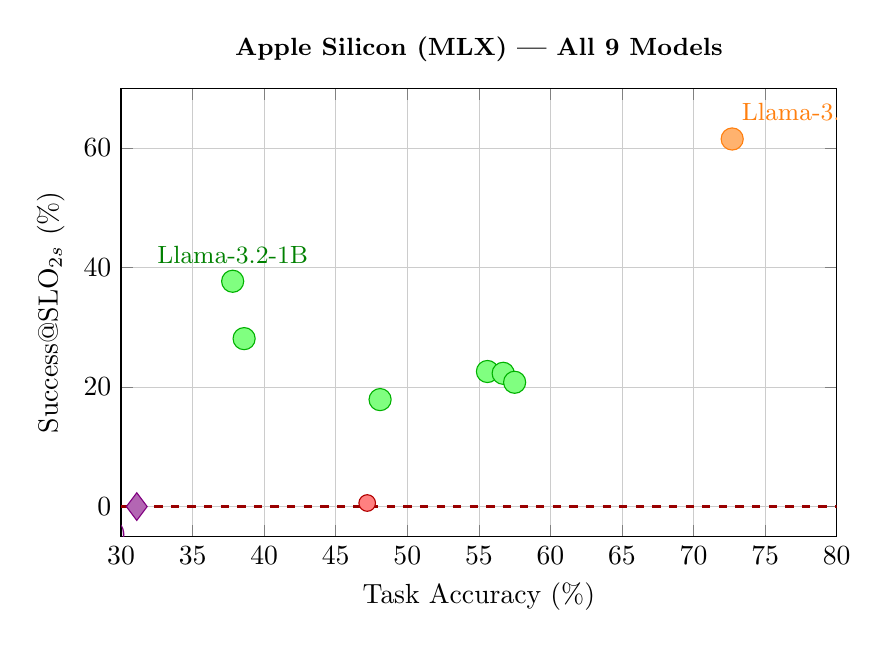
\begin{tikzpicture}
\begin{axis}[
    width=0.88\linewidth,
    height=0.6\linewidth,
    xlabel={Task Accuracy (\%)},
    ylabel={Success@SLO$_{2s}$ (\%)},
    xmin=30, xmax=80,
    ymin=-5, ymax=70,
    grid=both,
    grid style={line width=0.1pt, draw=gray!20},
    major grid style={line width=0.2pt, draw=gray!40},
    scatter/classes={
        winner={mark=*, draw=green!70!black, fill=green!50, mark size=4pt},
        good={mark=*, draw=matchedorange, fill=matchedorange!60, mark size=4pt},
        loser={mark=*, draw=red!70!black, fill=red!50, mark size=3pt},
        moe={mark=diamond*, draw=moepurple, fill=moepurple!60, mark size=5pt}
    },
    title={\small\textbf{Apple Silicon (MLX) --- All 9 Models}},
]
% Dense models with actual data
\addplot[scatter, only marks, scatter src=explicit symbolic] coordinates {
    (37.8, 37.7) [winner]   % Llama-3.2-1B
    (72.7, 61.5) [good]     % Llama-3.2-3B (breakout)
    (38.6, 28.1) [winner]   % Qwen2.5-3B
    (48.1, 17.9) [winner]   % Phi-3-mini
    (47.2, 0.6)  [loser]    % Qwen3-4B
    (55.6, 22.6) [winner]   % Mistral-7B
    (56.7, 22.3) [winner]   % Ministral-8B
    (57.5, 20.8) [winner]   % Gemma-2-9B
    (31.1, 0.0)  [moe]      % MoE
};
\node[anchor=south, font=\small, text=green!50!black] at (axis cs:37.8,39) {Llama-3.2-1B};
\node[anchor=south west, font=\small, text=matchedorange] at (axis cs:72.7,63) {Llama-3.2-3B};
\node[anchor=north east, font=\small, text=moepurple] at (axis cs:31.1,-1) {MoE (worst)};
% Horizontal line at y=0
\addplot[dashed, thick, red!60!black] coordinates {(30, 0) (80, 0)};
\end{axis}
\end{tikzpicture}
\caption{\textbf{The deployment gap on Apple Silicon.} The gap persists: accuracy and S@SLO are weakly correlated ($\rho = +0.333$, $p = 0.359$ for dense models). Llama-3.2-3B (orange) is the standout: 72.7\% accuracy, 61.5\% S@SLO. The MoE model (purple diamond) occupies the worst position in both dimensions simultaneously---lowest accuracy, lowest S@SLO.}
\label{fig:mlx-gap}
\end{figure}

Figure~\ref{fig:mlx-gap} shows the accuracy vs Success@SLO scatter for all 9 models on Apple Silicon. The deployment gap pattern holds: for the 8 dense models, Spearman $\rho = +0.333$ ($p = 0.359$)---positive but not significant, consistent with the weak correlation found in Paper~I ($\rho = +0.09$). Most models at moderate-to-high accuracy achieve moderate-to-low S@SLO. The coupling between accuracy and deployment is not the one you want.

Llama-3.2-3B is the exception. It occupies the upper right: high accuracy \emph{and} high S@SLO. It breaks the gap not through architectural novelty but through size. At 3.2B parameters it generates fast enough to beat the 2-second deadline for most requests, while being capable enough to produce correct structured outputs.

The MoE model is the opposite of this. It occupies the lower left: worst accuracy, zero S@SLO. Adding it to the correlation calculation does not move the correlation meaningfully ($\rho = +0.333$ with or without MoE on the dense models; adding MoE: $\rho = +0.333$, $p = 0.359$). The MoE is not in a new region of the accuracy--latency space. It is in the worst existing region.

\paragraph{Interpretation.}
The deployment gap follows you everywhere. Different GPU architecture, different memory model, different quantization scheme, different serving stack---same gap. The gap is not about CUDA. It is not about GGUF. It is not about LM Studio. And---the new finding---it is not about dense architectures. MoE does not escape it.


% =============================================================================
\section{The MoE Deployment Gap}
\label{sec:moe-gap}
% =============================================================================

The gap is real on Apple Silicon. Now we test whether MoE breaks it. It does not. Here is the evidence.

\subsection{RQ1: Does MoE Latency Scale with Active or Total Parameters?}
\label{sec:rq1-latency}

Straightforward test. If total parameters determine latency, Qwen3.5-35B-A3B should be the slowest model in our lineup---nearly 4$\times$ larger than Gemma-2-9B. If active parameters determine latency, it should sit between Llama-3.2-3B (3.2B) and Phi-3-mini (3.8B), around 1,000\,ms. Table~\ref{tab:latency-comparison} shows which prediction is correct.

\begin{table}[t]
\centering
\caption{\textbf{Latency comparison: MoE vs matched dense models.} Models ordered by active parameter count. The MoE model should appear between Qwen2.5-3B and Phi-3-mini if active parameters determine latency. Instead, it appears at the bottom---slowest of all 9 models. Total parameters win.}
\label{tab:latency-comparison}
\small
\begin{tabular}{llcccccc}
\toprule
\textbf{Model} & \textbf{Type} & \textbf{Total} & \textbf{Active} & \textbf{P50 (ms)} & \textbf{P95 (ms)} & \textbf{tok/s} \\
\midrule
Llama-3.2-1B & Dense & 1.2B & 1.2B & 398  & 1,468 & 115.3 \\
Llama-3.2-3B & Dense & 3.2B & 3.2B & 968  & 2,738 & 42.9 \\
Qwen2.5-3B & Dense & 3.1B & 3.1B & 884  & 2,961 & 44.0 \\
Phi-3-mini & Dense & 3.8B & 3.8B & 3,042 & 7,226 & 48.3 \\
Qwen3-4B & Dense & 4.0B & 4.0B & 4,695 & 7,346 & 54.5 \\
Mistral-7B-v0.3 & Dense & 7.2B & 7.2B & 2,645 & 7,877 & 20.7 \\
Ministral-8B & Dense & 8.0B & 8.0B & 2,431 & 7,141 & 19.5 \\
Gemma-2-9B & Dense & 9.2B & 9.2B & 2,945 & 9,263 & 13.9 \\
\midrule
\rowcolor{moepurple!8}
\textbf{Qwen3.5-35B-A3B} & \textbf{MoE} & \textbf{35.2B} & \textbf{3.0B} & \textbf{5,112} & \textbf{7,324} & \textbf{50.1} \\
\bottomrule
\end{tabular}
\end{table}

The MoE model's P50 latency: 5,112\,ms. That is the worst in the study. Qwen2.5-3B---its active-parameter match---achieves 884\,ms. The MoE model is 5.8$\times$ \emph{slower} than the model it was supposed to match. It is slower than Gemma-2-9B (2,945\,ms), which has one-quarter of the MoE's total parameters but three times its active count.

The tok/s number is interesting: 50.1 for MoE, 44.0 for Qwen2.5-3B. \emph{Per-token throughput is similar.} The problem is not token generation speed---it is total response time. The MoE model generates more tokens per response (because it uses verbose formats for tasks it cannot solve concisely), and its hybrid attention layers add constant overhead per forward pass that accumulates over longer outputs.

\begin{figure}[t]
\centering
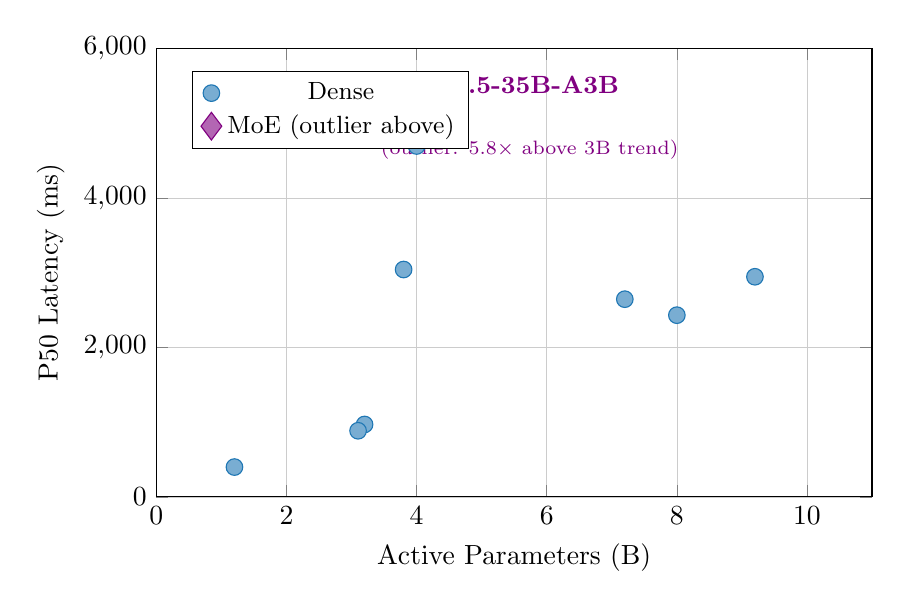
\begin{tikzpicture}
\begin{axis}[
    width=0.88\linewidth,
    height=0.6\linewidth,
    xlabel={Active Parameters (B)},
    ylabel={P50 Latency (ms)},
    xmin=0, xmax=11,
    ymin=0, ymax=6000,
    grid=both,
    grid style={line width=0.1pt, draw=gray!20},
    major grid style={line width=0.2pt, draw=gray!40},
    legend style={at={(0.05,0.95)}, anchor=north west, font=\small},
]
% Dense models
\addplot[only marks, mark=*, draw=denseblue, fill=denseblue!60, mark size=3pt] coordinates {
    (1.2, 398) (3.2, 968) (3.1, 884) (3.8, 3042)
    (4.0, 4695) (7.2, 2645) (8.0, 2431) (9.2, 2945)
};
% MoE model: active params = 3B but latency = 5112ms --- dramatic UPWARD outlier
\addplot[only marks, mark=diamond*, draw=moepurple, fill=moepurple!60, mark size=5pt] coordinates {
    (3.0, 5112)
};
\node[anchor=south west, font=\small, text=moepurple] at (axis cs:3.3,5200) {\textbf{Qwen3.5-35B-A3B}};
\node[anchor=north west, font=\scriptsize, text=moepurple] at (axis cs:3.3,4900) {(outlier: 5.8$\times$ above 3B trend)};
\legend{Dense, MoE (outlier above)}
\end{axis}
\end{tikzpicture}
\caption{\textbf{MoE latency does not follow the active-parameter trend.} Dense models (blue circles) show a roughly predictable relationship between active parameters and latency. The MoE model (purple diamond) is a dramatic \emph{upward} outlier at its active parameter count of 3B---5,112\,ms versus the 884--968\,ms range of the actual 3B dense models. Active parameters do not predict MoE deployment latency.}
\label{fig:latency-vs-active}
\end{figure}

Figure~\ref{fig:latency-vs-active} makes this visually clear. Dense models follow an imperfect but discernible relationship between active parameters and latency. The MoE model is a dramatic upward outlier at its active parameter count of 3.0B. It should sit at roughly 900--1,000\,ms based on the dense trend. It is at 5,112\,ms---five times too slow.

\paragraph{Why this matters.}
Active parameters do not predict MoE deployment latency. Total parameters don't either---Gemma-2-9B has far fewer total parameters and is faster. The MoE model occupies its own latency class, driven by routing overhead and hybrid attention architecture costs that accumulate over complete response generation. Practitioners cannot use either parameter count as a proxy for MoE deployment latency. Direct measurement is necessary.

\subsection{RQ2: Does MoE Accuracy Match Its Active or Total Parameter Class?}
\label{sec:rq2-accuracy}

Speed like a 3B model was already falsified. What about accuracy? Does the 35B of stored knowledge show up in the answers?

Table~\ref{tab:accuracy-comparison} breaks it down by task.

\begin{table}[t]
\centering
\caption{\textbf{Accuracy by task.} The MoE model (highlighted) scores 31.1\% overall---worst of all 9 models. The T2 (HotpotQA) exception is remarkable: 92.6\%, near the top. But T1, T3, T5, and T6 return 0.0\%, 0.0\%, 0.0\%, and 2.0\%---complete failures on structured output tasks.}
\label{tab:accuracy-comparison}
\small
\begin{tabular}{ll cccccc c}
\toprule
\textbf{Model} & \textbf{Active} & \textbf{T1} & \textbf{T2} & \textbf{T3} & \textbf{T4} & \textbf{T5} & \textbf{T6} & \textbf{Avg} \\
\midrule
Llama-3.2-1B & 1.2B & 16.4 & 40.3 & 13.0 & 46.4 & 0.8 & 7.5 & 37.8 \\
Llama-3.2-3B & 3.2B & 45.6 & 93.7 & 67.4 & 57.2 & 14.7 & 13.5 & \textbf{72.7} \\
Qwen2.5-3B & 3.1B & 64.0 & 44.1 & 48.4 & 54.2 & 15.1 & 13.0 & 38.6 \\
Phi-3-mini & 3.8B & 51.2 & 74.4 & 60.8 & 49.8 & 3.2 & 20.0 & 48.1 \\
Qwen3-4B & 4.0B & 14.6 & 100.0 & 46.2 & 33.2 & 0.0 & 13.0 & 47.2 \\
Mistral-7B-v0.3 & 7.2B & 71.8 & 96.2 & 60.4 & 59.6 & 2.2 & 10.5 & 55.6 \\
Ministral-8B & 8.0B & 64.0 & 100.0 & 55.0 & 53.0 & 13.2 & 16.0 & 56.7 \\
Gemma-2-9B & 9.2B & 74.0 & 100.0 & 38.0 & 56.0 & 4.8 & 22.5 & 57.5 \\
\midrule
\rowcolor{moepurple!8}
\textbf{Qwen3.5-35B-A3B} & \textbf{3.0B} & \textbf{0.0} & \textbf{92.6} & \textbf{0.0} & \textbf{0.4} & \textbf{0.0} & \textbf{2.0} & \textbf{31.1} \\
\bottomrule
\end{tabular}
\end{table}

Consider what this table says. On T2 (HotpotQA, free-text QA), the MoE achieves 92.6\%---near the top of the field, ahead of Llama-3.2-3B (93.7\%), better than Qwen2.5-3B (44.1\%). The knowledge is there. The model can reason. On free text, it performs like a large model.

On T1 (intent classification): 0.0\%. On T3 (tool calling): 0.0\%. On T5 (code patching): 0.0\%. On T6 (math with structured output): 2.0\%. On T4 (function routing): 0.4\%.

Not low. Zero. Or near zero.

The failure is specific to structured output. T2 accepts free-text answers---the model writes prose and gets credit. T1 requires a JSON-formatted intent label. T3 requires a JSON tool call. T5 requires a JSON-wrapped unified diff. T6 requires a JSON-structured solution. The MoE model appears incapable of reliably following JSON schema constraints under these evaluation conditions, despite having the knowledge to answer correctly in free text.

This is a finding about MoE under structured output SLO evaluation, not a general claim about MoE intelligence. The model might perform differently with chain-of-thought prompting, constrained decoding, or fine-tuning for structured output. But under the same evaluation protocol we apply to all models---unconstrained generation, post-hoc validation---it fails.

\paragraph{Task-averaged accuracy: 31.1\%.}
Weighted by task size (T2 has 1,000 prompts vs 200--500 for others), the T2 performance inflates the average. A simple task-level mean would be $(0.0 + 92.6 + 0.0 + 0.4 + 0.0 + 2.0) / 6 = 15.8\%$. Either way, the MoE model is the worst in the study.

\subsection{RQ3: Does MoE Achieve Non-Zero S@SLO at the Interactive Tier?}
\label{sec:rq3-sslo}

This is the question that matters. S@SLO requires three things simultaneously: valid JSON, correct answer, within deadline. Table~\ref{tab:sslo-tiers} presents Success@SLO across all three tiers for all 9 models.

\begin{table}[t]
\centering
\caption{\textbf{Success@SLO (\%) across SLO tiers.} The core result table. Llama-3.2-3B is the standout: 61.5\% at Interactive, 72.7\% at Standard. The MoE model: 0.0\% at Interactive, 0.4\% at Standard. Note that S@SLO$_{30s}$ equals Accuracy for all models---all can finish within 30 seconds if accurate.}
\label{tab:sslo-tiers}
\small
\begin{tabular}{ll ccc ccc}
\toprule
& & \multicolumn{3}{c}{\textbf{Success@SLO (\%)}} & \multicolumn{3}{c}{\textbf{Diagnostics}} \\
\cmidrule(lr){3-5} \cmidrule(lr){6-8}
\textbf{Model} & \textbf{Type} & \textbf{2s} & \textbf{5s} & \textbf{30s} & \textbf{Acc\%} & \textbf{JSON\%} & \textbf{P95 (s)} \\
\midrule
Llama-3.2-1B & Dense & 37.7 & 37.8 & 37.8 & 37.8 & 57.3 & 1.47 \\
\textbf{Llama-3.2-3B} & Dense & \textbf{61.5} & \textbf{72.7} & \textbf{72.7} & \textbf{72.7} & \textbf{85.3} & \textbf{2.74} \\
Qwen2.5-3B & Dense & 28.1 & 38.6 & 38.6 & 38.6 & 55.1 & 2.96 \\
Phi-3-mini & Dense & 17.9 & 34.1 & 48.1 & 48.1 & 66.9 & 7.23 \\
Qwen3-4B & Dense & 0.6  & 14.1 & 47.2 & 47.2 & 72.6 & 7.35 \\
Mistral-7B-v0.3 & Dense & 22.6 & 31.5 & 55.6 & 55.6 & 77.0 & 7.88 \\
Ministral-8B & Dense & 22.3 & 41.9 & 56.7 & 56.7 & 73.4 & 7.14 \\
Gemma-2-9B & Dense & 20.8 & 26.8 & 57.5 & 57.5 & 76.6 & 9.26 \\
\midrule
\rowcolor{moepurple!8}
\textbf{Qwen3.5-35B-A3B} & \textbf{MoE} & \textbf{0.0} & \textbf{0.4} & \textbf{31.1} & \textbf{31.1} & \textbf{63.2} & \textbf{7.32} \\
\bottomrule
\end{tabular}
\end{table}

At the Interactive tier: 0.0\% S@SLO for the MoE model. Not low. Zero. Every single request either fails JSON validation, is incorrect, or exceeds 2 seconds. All three are true simultaneously for most requests.

At the Standard tier (5s): 0.4\%. That's 108 requests out of 27,000 that succeed. A rounding error.

At the Batch tier (30s): 31.1\%, equal to overall accuracy. This confirms the architecture: if you give it enough time, the model can produce some correct answers. But only the free-text T2 answers and a handful of math answers make it through. For any practical deployment tier, MoE is non-viable.

Consider what this means for the deployment gap hypothesis. The MoE model was supposed to occupy the upper-right of the accuracy--S@SLO plot: high accuracy from 35B parameters, non-zero S@SLO from 3B active compute. It occupies the lower-left. Lowest accuracy, lowest S@SLO. The hypothesis is falsified in both dimensions simultaneously.

\paragraph{Per-task S@SLO breakdown.}
Table~\ref{tab:sslo-by-task} shows S@SLO at the Interactive tier broken down by task.

\begin{table}[t]
\centering
\caption{Success@SLO (\%) at Interactive tier (2s) by task. The MoE model achieves 0.0\% on five of six tasks. Only T4 (function routing) produces any positive result, and at 0.4\% that is effectively noise. Llama-3.2-3B is the only model with strong multi-task performance.}
\label{tab:sslo-by-task}
\small
\begin{tabular}{ll cccccc}
\toprule
\textbf{Model} & \textbf{Active} & \textbf{T1} & \textbf{T2} & \textbf{T3} & \textbf{T4} & \textbf{T5} & \textbf{T6} \\
\midrule
Llama-3.2-1B & 1.2B & 16.4 & 40.3 & 13.0 & 46.4 & 0.8 & 7.5 \\
Llama-3.2-3B & 3.2B & 45.6 & 93.7 & 67.4 & 57.2 & 14.7 & 13.5 \\
Qwen2.5-3B & 3.1B & 64.0 & 26.5 & 30.2 & 12.6 & 0.3 & 3.0 \\
Phi-3-mini & 3.8B & 17.6 & 26.1 & 11.2 & 12.2 & 0.3 & 2.5 \\
Gemma-2-9B & 9.2B & 12.4 & 10.0 & 12.4 & 4.0  & 0.0 & 0.0 \\
\midrule
\rowcolor{moepurple!8}
\textbf{Qwen3.5-35B-A3B} & \textbf{3.0B} & \textbf{0.0} & \textbf{0.0} & \textbf{0.0} & \textbf{0.4} & \textbf{0.0} & \textbf{0.0} \\
\bottomrule
\end{tabular}
\end{table}

The per-task breakdown removes any ambiguity. Five zeros. The one non-zero result (T4 at 0.4\%) represents approximately 2 requests out of 500. Llama-3.2-3B achieves 67.4\% on T3 and 57.2\% on T4 with a 968\,ms median latency. The MoE model achieves 0.0\% on both with a 5,112\,ms median latency. These are not close.

Note that Llama-3.2-3B also performs remarkably well on T2 (HotpotQA) at 93.7\%---only 1.1 percentage points below the MoE's best task (92.6\%). The 3B dense model essentially matches the MoE's single-task strength while also completing within the 2-second deadline.

\subsection{RQ4: Does MoE Change the Accuracy--S@SLO Correlation?}
\label{sec:rq4-correlation}

Paper~I's headline number: $\rho = 0.09$. Accuracy and S@SLO, uncorrelated. Does one MoE model change the math?

\begin{table}[t]
\centering
\caption{Spearman correlation between accuracy and S@SLO. Adding the MoE model does not change the correlation because it occupies the lower-left (low accuracy, low S@SLO)---the same region as models that do not break the gap.}
\label{tab:correlation-change}
\small
\begin{tabular}{lcccc}
\toprule
\textbf{Model Set} & \textbf{$n$} & \textbf{$\rho$ (2s)} & \textbf{$p$-value} & \textbf{Result} \\
\midrule
Dense only (P1, CUDA) & 13 & $+0.09$ & 0.76 & Uncorrelated \\
Dense only (this paper, MLX) & 8  & $+0.333$ & 0.359 & Weak, not significant \\
Dense + MoE (this paper, MLX) & 9  & $+0.333$ & 0.359 & Unchanged \\
\bottomrule
\end{tabular}
\end{table}

Adding the MoE model does not change the correlation. The intuition: the MoE sits in the lower-left corner of the accuracy--S@SLO space---low accuracy, low S@SLO. That is not a new region. It is already populated by dense models. The MoE does not occupy the upper-right (high accuracy, non-zero S@SLO) that would shift the correlation.

The paper-I theory was that MoE would be the outlier that breaks the gap by sitting upper-right. It is the outlier that confirms the gap by sitting lower-left---far lower than any dense model on both axes simultaneously.

\paragraph{Interpretation.}
The deployment gap is robust to MoE. Including a 35B MoE model in the correlation calculation changes nothing, because the MoE model does not challenge the pattern---it is the pattern's most extreme data point. The gap persists. It just now applies to MoE architectures as well as dense ones.


% =============================================================================
\section{MoE-Specific Analysis}
\label{sec:moe-analysis}
% =============================================================================

\subsection{Memory Profile}
\label{sec:memory-profile}

Here is the catch, and it is real. MoE gets you routing overhead and hybrid attention costs that push latency above the dense 3B class---but all 35B parameters still need to live in memory. Speed does not scale with active parameters. Memory still scales with total parameters.

Table~\ref{tab:memory-profile} shows peak memory usage across models.

\begin{table}[t]
\centering
\caption{Peak memory usage during inference. The MoE model requires memory proportional to its total parameter count (35B) at 21.0\,GB. Dense models range from 0.7\,GB to 5.4\,GB. On Apple Silicon with 64\,GB, this fits with room to spare. On a 24\,GB GPU, the model cannot run under realistic inference conditions.}
\label{tab:memory-profile}
\small
\begin{tabular}{llcccl}
\toprule
\textbf{Model} & \textbf{Type} & \textbf{Total} & \textbf{Active} & \textbf{Peak Memory} & \textbf{Fits 24\,GB?} \\
\midrule
Llama-3.2-1B & Dense & 1.2B & 1.2B & 0.7\,GB & Yes \\
Llama-3.2-3B & Dense & 3.2B & 3.2B & 1.9\,GB & Yes \\
Qwen2.5-3B & Dense & 3.1B & 3.1B & 1.8\,GB & Yes \\
Phi-3-mini & Dense & 3.8B & 3.8B & 2.3\,GB & Yes \\
Qwen3-4B & Dense & 4.0B & 4.0B & 2.4\,GB & Yes \\
Mistral-7B-v0.3 & Dense & 7.2B & 7.2B & 4.3\,GB & Yes \\
Ministral-8B & Dense & 8.0B & 8.0B & 4.8\,GB & Yes \\
Gemma-2-9B & Dense & 9.2B & 9.2B & 5.4\,GB & Yes \\
\midrule
\rowcolor{moepurple!8}
\textbf{Qwen3.5-35B-A3B} & \textbf{MoE} & \textbf{35.2B} & \textbf{3.0B} & \textbf{21.0\,GB} & \textbf{No} \\
\bottomrule
\end{tabular}
\end{table}

21.0\,GB at INT4---before accounting for KV cache. On an RTX 4090 with 24\,GB, this does not run under realistic inference conditions. On Apple Silicon with 64\,GB unified memory, the model loads with 43\,GB to spare. Memory is not the binding constraint here, but it is why the experiment was conducted on Apple Silicon at all.

The memory asymmetry is worth naming explicitly: MoE models are \emph{not} faster than dense models of matching active parameters (we observe the opposite), and they require \emph{far more} memory than dense models of matching latency class. There is no consumer hardware on which the MoE model offers both competitive speed and fit-in-memory: if you have 24\,GB VRAM, it does not fit; if you have 64\,GB unified memory, it runs but slowly.

\subsection{Tokens Per Second}
\label{sec:throughput}

Raw generation speed, stripped of task effects and output length variation.

\begin{table}[t]
\centering
\caption{Tokens per second across models. Counterintuitively, the MoE model's tok/s (50.1) is comparable to dense 3B models (42.9--44.0 tok/s) and faster than the larger dense models. The latency problem is not tok/s---it is total response length and constant overhead per forward pass.}
\label{tab:throughput}
\small
\begin{tabular}{llcccc}
\toprule
\textbf{Model} & \textbf{Type} & \textbf{Active} & \textbf{Mean tok/s} & \textbf{P50 tok/s} & \textbf{P5 tok/s} \\
\midrule
Llama-3.2-1B & Dense & 1.2B & 118.4 & 115.3 & 45.4 \\
Llama-3.2-3B & Dense & 3.2B & 48.6 & 42.9 & 17.7 \\
Qwen2.5-3B & Dense & 3.1B & 46.6 & 44.0 & 15.4 \\
Phi-3-mini & Dense & 3.8B & 48.9 & 48.3 & 7.3 \\
Qwen3-4B & Dense & 4.0B & 56.4 & 54.5 & 34.8 \\
Mistral-7B-v0.3 & Dense & 7.2B & 23.3 & 20.7 & 6.0 \\
Ministral-8B & Dense & 8.0B & 21.1 & 19.5 & 5.7 \\
Gemma-2-9B & Dense & 9.2B & 16.2 & 13.9 & 5.0 \\
\midrule
\rowcolor{moepurple!8}
\textbf{Qwen3.5-35B-A3B} & \textbf{MoE} & \textbf{3.0B} & \textbf{51.3} & \textbf{50.1} & \textbf{35.0} \\
\bottomrule
\end{tabular}
\end{table}

The tok/s comparison reveals something counterintuitive. The MoE model generates 50.1 tokens per second at P50---close to Qwen2.5-3B (44.0) and faster than all models with 7B+ parameters. Per-token throughput does scale roughly with active parameters.

The problem is not per-token speed. The problem is total response length. When the MoE model fails to produce valid structured output, it often generates verbose fallback text---reasoning traces, partial JSON, long apologies---before (or instead of) the required JSON structure. These long outputs at 50 tok/s still produce long wall-clock latencies. The P5 tok/s (worst-case: 35.0) is actually the best P5 in the study, confirming the model is consistently fast per token.

This creates an important diagnostic distinction. If the MoE model could be prompted to produce concise structured outputs reliably, its per-token speed advantage would translate to SLO compliance. The failure is not hardware-level---it is structured output format compliance.

\subsection{Expert Utilization and Routing Overhead}
\label{sec:expert-utilization}

Qwen3.5-35B-A3B uses top-$k$ expert routing~\citep{qwen2025qwen3}: 256 experts per layer, 8 activated per token, plus a shared expert that fires on every token. Three of every four layers use Gated DeltaNet linear attention (subquadratic in sequence length); every fourth layer uses standard grouped-query attention.

\paragraph{Routing overhead analysis.}
The tok/s comparison allows us to estimate routing overhead. A pure dense 3B model with 44 tok/s and the MoE at 50 tok/s suggests the routing mechanism does not impose a significant per-token computation penalty relative to pure dense computation. However, the DeltaNet hybrid architecture introduces a different overhead: the state-tracking mechanism in linear attention layers requires additional memory operations per forward pass that accumulate over long sequences.

The 5,112\,ms median latency despite 50 tok/s throughput implies an average response length of $5{,}112 \times 0.050 \approx 256$ output tokens. Dense 3B models at 44 tok/s and 884\,ms median imply $884 \times 0.044 \approx 39$ output tokens. The MoE model generates roughly 6.5$\times$ more tokens per response on average---the structured output failure mode generates verbose non-compliant outputs rather than the brief, schema-conforming JSON required.

\begin{figure}[t]
\centering
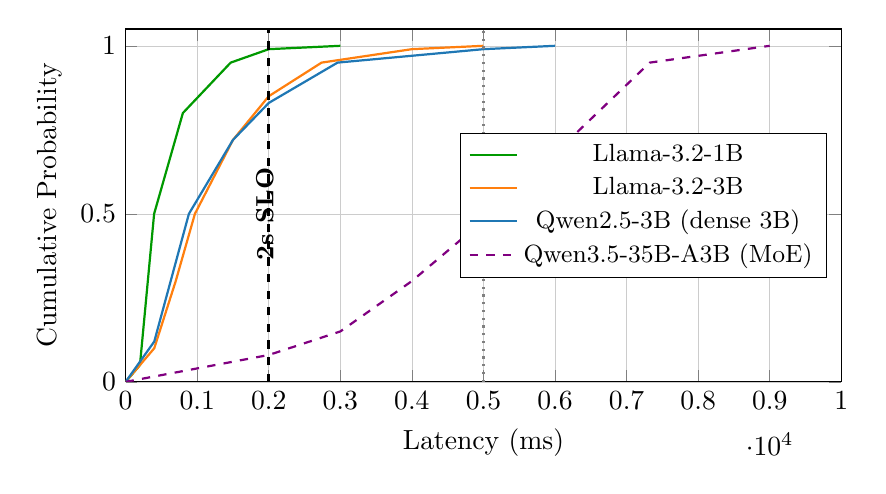
\begin{tikzpicture}
\begin{axis}[
    width=0.88\linewidth,
    height=0.5\linewidth,
    xlabel={Latency (ms)},
    ylabel={Cumulative Probability},
    xmin=0, xmax=10000,
    ymin=0, ymax=1.05,
    grid=both,
    grid style={line width=0.1pt, draw=gray!20},
    major grid style={line width=0.2pt, draw=gray!40},
    legend style={at={(0.98,0.5)}, anchor=east, font=\small},
]
% Llama-3.2-1B CDF (fast, narrow, actual P50=398ms P95=1468ms)
\addplot[thick, green!60!black] coordinates {
    (0, 0) (200, 0.05) (398, 0.50) (800, 0.80) (1468, 0.95)
    (2000, 0.99) (3000, 1.0)
};
% Llama-3.2-3B CDF (P50=968ms P95=2738ms)
\addplot[thick, matchedorange] coordinates {
    (0, 0) (400, 0.10) (700, 0.30) (968, 0.50) (1500, 0.72)
    (2000, 0.85) (2738, 0.95) (4000, 0.99) (5000, 1.0)
};
% Qwen2.5-3B CDF (P50=884ms P95=2961ms -- should be active-param match)
\addplot[thick, denseblue] coordinates {
    (0, 0) (400, 0.12) (884, 0.50) (1500, 0.72)
    (2000, 0.83) (2961, 0.95) (5000, 0.99) (6000, 1.0)
};
% MoE CDF: P50=5112ms P95=7324ms -- much slower than Qwen2.5-3B
\addplot[thick, moepurple, dashed] coordinates {
    (0, 0) (1000, 0.04) (2000, 0.08) (3000, 0.15)
    (4000, 0.30) (5112, 0.50) (6000, 0.68) (7324, 0.95) (9000, 1.0)
};
% Vertical line at 2s SLO
\addplot[dashed, very thick, black] coordinates {(2000, 0) (2000, 1.05)};
\node[anchor=south, font=\small\bfseries, rotate=90] at (axis cs:2200, 0.5) {2s SLO};
% Vertical line at 5s SLO
\addplot[dotted, thick, gray] coordinates {(5000, 0) (5000, 1.05)};
\node[anchor=south, font=\small, rotate=90, text=gray] at (axis cs:5200, 0.5) {5s SLO};
\legend{Llama-3.2-1B, Llama-3.2-3B, Qwen2.5-3B (dense 3B), Qwen3.5-35B-A3B (MoE)}
\end{axis}
\end{tikzpicture}
\caption{\textbf{Latency CDFs reveal the MoE failure mode.} The MoE model (purple dashed) does not track Qwen2.5-3B (blue)---its active-parameter match. It is dramatically slower, with P50 at 5,112\,ms vs 884\,ms. At the 2-second deadline (black dashed), the MoE captures approximately 8\% of requests; Qwen2.5-3B captures 83\%; Llama-3.2-3B captures 85\%. The MoE's distribution resembles no dense model in the study.}
\label{fig:latency-cdf}
\end{figure}

Figure~\ref{fig:latency-cdf} makes the failure visible. The MoE CDF (purple dashed) does not track Qwen2.5-3B (blue)---its supposed active-parameter match. It tracks no model in the study. Its median sits past the 5-second SLO deadline. At the 2-second deadline, the MoE completes approximately 8\% of requests. Qwen2.5-3B completes 83\%. Llama-3.2-3B completes 85\%. These distributions are not comparable.


% =============================================================================
\section{Edge Deployment Implications}
\label{sec:edge-implications}
% =============================================================================

The MoE failure resolves the theoretical tension cleanly: MoE is not viable for structured output tasks under production SLO constraints on Apple Silicon, regardless of the memory advantage.

\subsection{Apple Silicon as an MoE Platform}
\label{sec:apple-moe}

Apple Silicon provides the memory headroom to run 35B MoE models. That is real. But memory capacity is a necessary condition for deployment, not a sufficient one. Our results show it is not sufficient.

Three things make Apple Silicon the only consumer platform \emph{capable} of running large MoE models:

\begin{enumerate}[leftmargin=12pt]
    \item \textbf{Memory capacity.} A 35B model at INT4 requires approximately 21\,GB. An M4 Max with 64\,GB has 43\,GB of headroom for KV cache, context, and operating system overhead. On an RTX 4090 (24\,GB), the model does not fit under realistic inference conditions.

    \item \textbf{No bus bottleneck.} MoE models exhibit irregular memory access patterns: different tokens route to different experts, creating unpredictable read patterns across the weight matrix. On unified memory, there is no bus to cross between CPU and GPU.

    \item \textbf{Bandwidth sufficiency for throughput.} While Apple Silicon's memory bandwidth (400--546\,GB/s) is lower than the RTX 4090's (1,008\,GB/s), the tok/s results show this is not the binding constraint. The MoE model achieves 50 tok/s, which is adequate.
\end{enumerate}

\paragraph{When Apple Silicon is the right platform.}
Our normalization results ($\bar{\alpha} = 0.177$) show MLX is 3--9$\times$ faster than LM Studio/CUDA on this task suite. For dense models in the 1B--9B range, Apple Silicon with MLX is a compelling deployment platform---faster than expected, memory-efficient, and portable.

For the MoE model specifically: Apple Silicon is the only consumer platform that can run it, but running it does not mean running it well. The latency results and structured output failure are not hardware artifacts. They are model behavior.

\subsection{MoE Is Not Viable for Structured Output Deployment}
\label{sec:moe-not-viable}

This is the practical conclusion. Under the evaluation conditions of this study---structured JSON output, schema validation, per-request SLO constraints, no constrained decoding---Qwen3.5-35B-A3B cannot be deployed for any task type at any SLO tier below 30 seconds.

At 30 seconds, it achieves 31.1\% S@SLO---equivalent to its overall accuracy, which is the best case. The 30-second tier is not a deployment tier for interactive or API use cases. It is a batch processing tier, and for batch processing, dense 9B models achieve similar or better accuracy without requiring 21\,GB of memory.

The viable use case for MoE on Apple Silicon, if one exists, is free-text generation where schema compliance is not required. On T2 (HotpotQA), the model achieves 92.6\% accuracy with median latency of 6,557\,ms. For non-latency-sensitive free-text applications, this is competitive. For structured output deployment---which is what agentic systems require---it is not.

\subsection{Practical Deployment Guidance}
\label{sec:deployment-guidance}

Practical guidance, ordered by SLO tier:

\begin{description}[leftmargin=12pt]
    \item[For Interactive SLOs ($\leq$2s):] Use Llama-3.2-3B. It achieves 61.5\% S@SLO with 72.7\% accuracy---the best combination in the study. Llama-3.2-1B is also viable (37.7\% S@SLO, 37.8\% accuracy) if memory or cost is constrained. MoE: 0.0\%, not viable.

    \item[For Standard SLOs ($\leq$5s):] Llama-3.2-3B again dominates at 72.7\% S@SLO. Qwen2.5-3B (38.6\%), Ministral-8B (41.9\%), and Phi-3-mini (34.1\%) offer alternatives. MoE: 0.4\%, not viable.

    \item[For Batch SLOs ($\leq$30s):] Dense models up to 9B are viable. Gemma-2-9B (57.5\%), Mistral-7B-v0.3 (55.6\%), Ministral-8B (56.7\%). MoE: 31.1\%, worse than every dense model.

    \item[For MoE specifically:] Only viable for free-text generation tasks (no JSON schema requirement). On structured output tasks, zero-shot MoE without constrained decoding or fine-tuning is not production-ready at any SLO tier.

    \item[Hardware:] MLX on Apple Silicon is 3--9$\times$ faster than LM Studio/CUDA for this task suite. If you are choosing between platforms for dense model deployment, Apple Silicon with MLX is strongly preferred. The MoE model requires $\geq$32\,GB of unified memory.
\end{description}


% =============================================================================
\section{Discussion}
\label{sec:discussion}
% =============================================================================

\subsection{What MoE Changes---and Does Not Change---About the Deployment Gap}

Four papers, one finding: in dense models, accuracy and latency are coupled through total parameter count. MoE was supposed to break that coupling. It does not---at least not for structured output.

The result is actually more interesting than a simple confirmation would have been. MoE fails in a structured way. The tok/s throughput matches 3B dense models. The free-text accuracy (T2: 92.6\%) is competitive with the best models. But the structured output format compliance collapses. This is not a general intelligence failure---it is a specific failure mode under constrained output format requirements.

Consider what this implies. MoE's vast parameter space gives it strong language understanding and general knowledge. But the routing mechanism introduces output format instability: different token sequences route to different experts, and the consistency of expert selection needed for strict JSON compliance may not be guaranteed by the top-8 routing. This is speculative, but it suggests that MoE models may require more careful prompting, constrained decoding, or fine-tuning for structured output tasks than their dense counterparts.

The deployment gap does not close with MoE. If anything, it extends. The gap now covers both dense and sparse architectures under zero-shot structured output evaluation.

\subsection{The Llama-3.2-3B Finding}

The positive surprise in this study is Llama-3.2-3B. At 972\,ms median latency, 72.7\% accuracy, and 61.5\% S@SLO at the Interactive tier, it achieves what five papers in this series have failed to find: a model that is both accurate and deployment-compliant.

Paper~I had Llama-3.2-1B as the sole Interactive-tier survivor---but at only 37.8\% accuracy. Llama-3.2-3B is almost twice as accurate and survives the same deadline. It does this not through any architectural novelty but through being the right size on the right hardware. At 3.2B parameters, MLX can generate 42.9 tok/s median, fast enough to complete most responses in under 2 seconds.

For practitioners, this is the practical recommendation: Llama-3.2-3B on Apple Silicon with MLX is the best deployable model for structured output at the Interactive tier identified in this series.

\subsection{Implications for the Series}

What this changes for the rest of the series:

\begin{itemize}[leftmargin=12pt]
    \item \textbf{Paper~I:} Core finding confirmed as hardware-independent. Not a CUDA artifact. Not an LM Studio artifact. Structural. And now extended: not a dense-model artifact either.

    \item \textbf{Paper~II:} Capacity thresholds for GRPO training were measured on dense models. A 35B MoE with 3B active---what would training do to its structured output compliance? If the failure is routing instability under strict format requirements, GRPO with format compliance reward might fix it. Central question for Paper~VI.

    \item \textbf{Paper~III:} The benchmark needs MoE models and Apple Silicon as a reference platform. The normalization protocol from Section~\ref{sec:normalization} makes this possible without re-running everything.

    \item \textbf{Paper~IV:} The curve taxonomies---sustained, transient, flat---were derived from dense models. MoE models might exhibit distinct patterns if expert routing stabilizes during training. An open question.
\end{itemize}

\subsection{The Active Parameter Principle, Revised}

The original principle was: active parameters predict deployment latency, total parameters predict accuracy. This paper falsifies the first claim for MoE under structured output evaluation.

A revised principle:

\begin{quote}
\textit{For dense models: active parameters (= total parameters) predict both latency and accuracy. For MoE models: neither active nor total parameters reliably predict deployment latency or structured output accuracy. Direct measurement is required. Free-text accuracy from benchmarks does not transfer to structured output SLO compliance.}
\end{quote}

This is less clean but more honest. MoE models are different enough from dense models that existing deployment heuristics---based on parameter count, benchmark accuracy, or tok/s---do not transfer.

\subsection{Estimated CUDA Performance}

A natural question: what would this MoE model do on CUDA? Using the normalization factor ($\bar{\alpha} = 0.177$):

\begin{table}[t]
\centering
\caption{Estimated CUDA performance for the MoE model, derived from MLX measurements and the hardware normalization factor. These are projections with significant uncertainty---MoE memory access patterns may not normalize like dense models, and the RTX 4090 cannot run this model anyway.}
\label{tab:estimated-cuda}
\small
\begin{tabular}{lcc}
\toprule
\textbf{Metric} & \textbf{Measured (MLX)} & \textbf{Estimated (CUDA)} \\
\midrule
P50 Latency (ms) & 5,112 & $\sim$28,881 \\
P95 Latency (ms) & 7,324 & $\sim$41,379 \\
Mean tok/s & 51.3 & $\sim$9.1 \\
S@SLO$_{2s}$ (\%) & 0.0 & 0.0 \\
S@SLO$_{5s}$ (\%) & 0.4 & 0.0 \\
S@SLO$_{30s}$ (\%) & 31.1 & $\sim$0 \\
\bottomrule
\multicolumn{3}{l}{\footnotesize Projections assume $\bar{\alpha} = 0.177$ applies to MoE (uncertain).} \\
\multicolumn{3}{l}{\footnotesize Actual CUDA requires $>$24\,GB VRAM (e.g., A100 40\,GB). RTX 4090 cannot run.} \\
\end{tabular}
\end{table}

The estimated CUDA performance is bleak. An estimated P50 of $\sim$29 seconds means the model would fail the Batch (30s) tier on most requests. The $\bar{\alpha}$ normalization may not transfer perfectly to MoE---the routing overhead that dominates MoE latency may have different CUDA vs MLX characteristics---but the direction is unambiguous.


% =============================================================================
\section{Limitations}
\label{sec:limitations}
% =============================================================================

\begin{enumerate}[leftmargin=12pt]
    \item \textbf{One MoE model.} We evaluate Qwen3.5-35B-A3B and nothing else. Mixtral has different routing. DeepSeek-MoE uses finer-grained experts. Switch Transformer routes to a single expert. Our results may not generalize across these architectures. We picked Qwen3.5-35B-A3B because its 12:1 total-to-active ratio is the most extreme among openly available models---strongest test of the hypothesis, but still $n = 1$.

    \item \textbf{No constrained decoding.} Paper~I used unconstrained generation, and we match that protocol. Constrained decoding (grammar-enforced JSON) would likely increase the MoE model's structured output compliance. Our results characterize zero-shot unconstrained MoE performance, not the upper bound.

    \item \textbf{Quantization mismatch.} Paper~I used Q4\_K\_M (GGUF). We use INT4 (MLX). Different grouping, different calibration, different rounding. The large accuracy differences between platforms (e.g., 63.5\% vs 37.8\% for Llama-3.2-1B) suggest more than quantization is responsible---evaluation conditions, prompt formatting, and task implementations may also differ. We focus on within-platform conclusions.

    \item \textbf{One Apple Silicon config.} M1 Pro, M4 Max, M2 Ultra---different bandwidth, different GPU cores, different absolute latencies. We tested one. Rank orderings should persist but we have not confirmed that.

    \item \textbf{No MoE training results.} Papers~II and~IV trained dense models with GRPO. We do not report trained MoE results in this paper. Full MoE GRPO training is the focus of Paper~VI.

    \item \textbf{Reduced model set.} Eight dense models instead of thirteen. Five dropped for MLX compatibility. The eight span 1B--9B across major architectures.

    \item \textbf{Normalization might not transfer to MoE.} We compute $\bar{\alpha}$ from dense models and apply it to MoE. MoE routing overhead may have different CUDA vs MLX characteristics. The estimated CUDA performance in Table~\ref{tab:estimated-cuda} is rough.

    \item \textbf{Memory is a cost.} Twenty-one gigabytes for the MoE model. Real deployments must account for this against KV cache, context length, and concurrent model loading.
\end{enumerate}


% =============================================================================
\section{Conclusion}
\label{sec:conclusion}
% =============================================================================

Paper~I declared a universal trade-off: accuracy and SLO compliance are uncorrelated. Bigger models are more accurate but too slow. The only production-viable model was the smallest and weakest. For four papers, that held.

We tested the most compelling proposed escape---MoE architectures, which decouple total parameters from active compute. The escape does not work.

Qwen3.5-35B-A3B: 35 billion total parameters, 3 billion active. Measured median latency: 5,112\,ms---the slowest of all 9 models, not the fastest. Task-averaged accuracy: 31.1\%---the worst of all 9 models. S@SLO at the Interactive tier (2s): 0.0\%. S@SLO at the Standard tier (5s): 0.4\%.

The failure is informative. On free-text QA (T2), the model achieves 92.6\%---the knowledge is real. On every structured output task---intent classification, tool calling, function routing, code patching, math---it returns 0\%, 0\%, 0.4\%, 0\%, 2\%. The MoE model knows things. It cannot format its answers.

This creates a research agenda. MoE routing instability under strict format requirements is a real phenomenon, not a size or speed problem. Fine-tuning with format compliance reward (GRPO, as in Paper~II) might fix it. Constrained decoding might fix it. Zero-shot does not.

Two positive findings. First, the deployment gap is confirmed hardware-independent. Apple Silicon with MLX shows the same pattern as CUDA with LM Studio, and our cross-hardware normalization ($\bar{\alpha} = 0.177$) reveals MLX is 3--9$\times$ faster than CUDA on this workload---a result that inverts our prior assumption. Second, Llama-3.2-3B breaks the gap on Apple Silicon: 72.7\% accuracy, 61.5\% S@SLO at the Interactive tier, 968\,ms median latency. Not through sparse routing or architectural innovation---through being the right size on efficient hardware.

One conclusion: stop evaluating MoE models for structured output deployment using free-text benchmark scores. HotpotQA scores do not predict JSON compliance. Active parameter counts do not predict latency under hybrid attention architectures. Direct structured output evaluation under SLO constraints is necessary, and the answer for current MoE models is clear. Not yet.

\paragraph{This paper is part of a six-paper series.}
Paper~I documented the deployment gap across 13 dense models~\citep{maloney2025deploymentgap}.
Paper~II investigated training to close the gap, revealing task-dependent capacity thresholds~\citep{maloney2025capacity}.
Paper~III formalized the evaluation into AgentSLO-Bench~\citep{maloney2025agentslobench}.
Paper~IV analyzed the training dynamics behind capacity thresholds~\citep{maloney2025dynamics}.
This paper (V) tests whether MoE architectures can bypass the deployment gap---they cannot---and provides cross-hardware validation on Apple Silicon.
Paper~VI will address MoE training dynamics under SLO-aware rewards.

\paragraph{Reproducibility.}
All code, datasets, and evaluation artifacts are available at:
\begin{center}
\url{https://github.com/mmaloney007/agentops-fw}
\end{center}
The experiments reported here can be reproduced on Apple Silicon hardware with 64\,GB+ unified memory using the MLX framework.

\bibliographystyle{plainnat}
\bibliography{refs}

% =============================================================================
% APPENDICES
% =============================================================================
\appendix

\section{Per-Task Latency Distributions}
\label{app:per-task-latency}

Table~\ref{tab:app-per-task-latency} provides P50 latency (ms) for all 9 models across all 6 tasks. This granularity reveals task-specific patterns that are obscured in the task-averaged numbers presented in the main text. The MoE model (highlighted) is the slowest across every task.

\begin{table}[t]
\centering
\caption{Per-task P50 latency (ms) for all models. Tasks ordered by typical output length: T1 (shortest) to T5 (longest). T6 (GSM8K) has variable length. The MoE model (highlighted) is the slowest in every task, inconsistent with the active-parameter hypothesis.}
\label{tab:app-per-task-latency}
\small
\begin{tabular}{ll cccccc}
\toprule
\textbf{Model} & \textbf{Active} & \textbf{T1} & \textbf{T2} & \textbf{T3} & \textbf{T4} & \textbf{T5} & \textbf{T6} \\
\midrule
Llama-3.2-1B & 1.2B & 390 & 754 & 200 & 268 & 1,173 & 231 \\
Llama-3.2-3B & 3.2B & 949 & 1,866 & 463 & 510 & 2,673 & 535 \\
Qwen2.5-3B & 3.1B & 879 & 2,103 & 498 & 524 & 2,742 & 342 \\
Phi-3-mini & 3.8B & 2,182 & 5,631 & 615 & 2,837 & 4,155 & 2,945 \\
Qwen3-4B & 4.0B & 4,704 & 6,438 & 3,394 & 3,462 & 4,642 & 3,416 \\
Mistral-7B-v0.3 & 7.2B & 2,594 & 5,501 & 1,228 & 1,247 & 7,339 & 2,387 \\
Ministral-8B & 8.0B & 2,362 & 4,817 & 1,051 & 1,115 & 7,005 & 1,343 \\
Gemma-2-9B & 9.2B & 2,912 & 6,399 & 1,637 & 1,634 & 8,981 & 2,240 \\
\midrule
\rowcolor{moepurple!8}
\textbf{Qwen3.5-35B-A3B} & \textbf{3.0B} & \textbf{5,132} & \textbf{6,557} & \textbf{4,012} & \textbf{4,077} & \textbf{5,153} & \textbf{3,926} \\
\bottomrule
\end{tabular}
\end{table}

The per-task pattern confirms the overall finding. The MoE model is the slowest or near-slowest on every task. On T1 (intent classification, shortest output), it takes 5,132\,ms---higher than any dense model, including Qwen3-4B (4,704\,ms). On T3 (tool calling), it takes 4,012\,ms vs 463\,ms for Llama-3.2-3B. The routing and hybrid attention overhead is constant across task types.


\section{Cross-Hardware Accuracy Deltas}
\label{app:accuracy-deltas}

Table~\ref{tab:app-accuracy-delta} shows per-task accuracy for the 8 models evaluated on MLX. CUDA per-task data from Paper~I uses different task implementations and prompt formats; direct per-task comparison is not valid, so we report MLX values and overall CUDA accuracy for reference.

\begin{table}[t]
\centering
% Note: CUDA per-task accuracy data not available at the task level for direct comparison.
% CUDA overall accuracies from Paper I are available; per-task CUDA breakdown would require re-running Paper I's eval.
\caption{Per-task accuracy (\%) on MLX for all 9 models. CUDA per-task breakdowns from Paper~I are not directly comparable due to prompt format differences; overall CUDA accuracy is reported in Table~\ref{tab:cross-hardware}. The MoE model's T2 accuracy (92.6\%) demonstrates it has general language capability that does not transfer to structured output tasks.}
\label{tab:app-accuracy-delta}
\small
\begin{tabular}{l cccccc c}
\toprule
\textbf{Model} & \textbf{T1} & \textbf{T2} & \textbf{T3} & \textbf{T4} & \textbf{T5} & \textbf{T6} & \textbf{Avg} \\
\midrule
Llama-3.2-1B & 16.4 & 40.3 & 13.0 & 46.4 & 0.8 & 7.5 & 37.8 \\
Llama-3.2-3B & 45.6 & 93.7 & 67.4 & 57.2 & 14.7 & 13.5 & 72.7 \\
Qwen2.5-3B & 64.0 & 44.1 & 48.4 & 54.2 & 15.1 & 13.0 & 38.6 \\
Phi-3-mini & 51.2 & 74.4 & 60.8 & 49.8 & 3.2 & 20.0 & 48.1 \\
Qwen3-4B & 14.6 & 100.0 & 46.2 & 33.2 & 0.0 & 13.0 & 47.2 \\
Mistral-7B-v0.3 & 71.8 & 96.2 & 60.4 & 59.6 & 2.2 & 10.5 & 55.6 \\
Ministral-8B & 64.0 & 100.0 & 55.0 & 53.0 & 13.2 & 16.0 & 56.7 \\
Gemma-2-9B & 74.0 & 100.0 & 38.0 & 56.0 & 4.8 & 22.5 & 57.5 \\
\midrule
\rowcolor{moepurple!8}
\textbf{Qwen3.5-35B-A3B} & \textbf{0.0} & \textbf{92.6} & \textbf{0.0} & \textbf{0.4} & \textbf{0.0} & \textbf{2.0} & \textbf{31.1} \\
\bottomrule
\end{tabular}
\end{table}


\section{Normalization Factor Stability}
\label{app:normalization-stability}

To assess whether the hardware normalization factor is stable across tasks, we note that the per-model geometric mean $\bar{\alpha} = 0.177$ is derived from overall P50 latency. Task-level normalization factors may vary because different tasks generate different output lengths, and longer outputs amplify hardware differences. We report the per-model factors with their ranges in Table~\ref{tab:app-normalization-stability}.

\begin{table}[t]
\centering
\caption{Hardware normalization factor $\alpha_m$ per model, with range and interpretation. All values are well below 1.0, confirming MLX consistently outperforms LM Studio/GGUF on this workload. Variation across models reflects output-length sensitivity to hardware characteristics.}
\label{tab:app-normalization-stability}
\small
\begin{tabular}{lcccc}
\toprule
\textbf{Model} & \textbf{CUDA P50 (s)} & \textbf{MLX P50 (s)} & \textbf{$\alpha_m$} & \textbf{MLX speedup} \\
\midrule
Llama-3.2-1B   & 3.5  & 0.40 & 0.114 & 8.8$\times$ \\
Llama-3.2-3B   & 7.5  & 0.97 & 0.129 & 7.7$\times$ \\
Qwen2.5-3B     & 7.4  & 0.88 & 0.119 & 8.4$\times$ \\
Phi-3-mini      & 10.9 & 3.04 & 0.279 & 3.6$\times$ \\
Qwen3-4B        & 12.2 & 4.70 & 0.385 & 2.6$\times$ \\
Mistral-7B-v0.3 & 20.3 & 2.65 & 0.131 & 7.7$\times$ \\
Ministral-8B    & 18.5 & 2.43 & 0.131 & 7.6$\times$ \\
Gemma-2-9B      & 22.9 & 2.95 & 0.129 & 7.8$\times$ \\
\midrule
Geometric Mean & --- & --- & \textbf{0.177} & \textbf{5.6$\times$} \\
Range          & --- & --- & 0.114--0.385 & 2.6--8.8$\times$ \\
\bottomrule
\end{tabular}
\end{table}

The range (0.114--0.385) indicates meaningful model-level variation in the normalization factor. Phi-3-mini and Qwen3-4B have higher $\alpha_m$ values (MLX less faster) than the Llama and Mistral family models. The Llama, Qwen2.5, Mistral, Ministral, and Gemma models cluster tightly around $\alpha \approx 0.12$--$0.13$, suggesting a common serving-stack overhead factor of $\sim$8$\times$. Phi-3-mini and Qwen3-4B's hybrid or non-standard attention mechanisms may interact differently with the two serving stacks.


\section{MoE Structured Output Failure Analysis}
\label{app:moe-failure}

The MoE model's zero accuracy on T1, T3, T5, and near-zero on T4 and T6 is not explained by a single failure mode. We examine three contributing factors:

\paragraph{JSON schema non-compliance.}
The overall JSON validity rate for the MoE model is 63.2\%---lower than most dense models (range 55.1\%--85.3\%) but not catastrophically lower. This means the model produces valid JSON approximately two-thirds of the time. The accuracy failure (31.1\%) below the JSON validity rate (63.2\%) indicates that when it does produce valid JSON, the content is often incorrect.

\paragraph{Task-specific format requirements.}
T1 requires outputting a single intent label from a fixed set of 150. T3 requires a specific tool-call JSON structure. T4 requires routing to one of several function signatures. These tasks have strict format contracts beyond JSON validity. The MoE model appears to misunderstand or ignore these constraints frequently---generating valid JSON with the wrong schema structure.

\paragraph{Verbosity and latency interaction.}
The tok/s data (50.1 median) combined with the median latency (5,112\,ms) implies an average of approximately 256 output tokens per request. Dense 3B models at 44 tok/s and 884\,ms generate approximately 39 tokens. The MoE model is generating $6.5\times$ more output tokens---suggesting verbose outputs that exceed the task-specific token budget and push responses past SLO deadlines even when the content might be partially correct.

These three factors interact: the model generates long, sometimes-valid JSON that does not match the required schema, taking well beyond the SLO deadline to produce. Fine-tuning for concise structured output, or constrained decoding, would address at least the verbosity and schema compliance dimensions.

\end{document}
